\section{Methodology}
Surface density is superior to volume density when it comes to local pointcloud quality assesment (PCQA). However, the process of determining surface density locally is computationally expensive and time consuming. This is not ideal for many applications, E.g. When trying to determine wether or not a rescan is necessary. This report proposes a novel method for estimating the local surface densities in a pointcloud with a neural network. This is especially usefull as the features used to predict the surface density can be calculated much faster than the suface density itself. 
To better understand the reason for choosing surface density as metric for local PCQA and how other features might reduce the complexity of its estimation, the problem is simplified to 2D and visualized in Figure~\ref{fig:area_and_circumference}. In the 2D point cloud, the points are uniformly distributed along the outline of the figure, resulting in equal local pointcloud quality (PCQ) across the figure. This can be determined by investigating the edge density at all points in the figure. Edge density is calculated as the number of points per unit length of edge, which involves estimating true length between all neighboring points along the edges. 
A simpler alternative is to draw circles around each point and count the number of neighboring points within the radius. This approach yields the local area density, which, as seen in Figure~\ref{fig:area_and_circumference}, is not ideal for evaluating PCQ, as it varies significantly depending on local geometry. Nonetheless, area density is strongly correlated with edge density, since the number of points inside the radius is the product of edge density and length of edge within the area. 
Even without computing the exact edge length within the radius, it is clear from the figure that certain geometrical attributes results in higher area densities than others. We call this geometry bias, and being able to estimate it is the cornerstone in this methodology.

\begin{figure}[H]
    \centering
    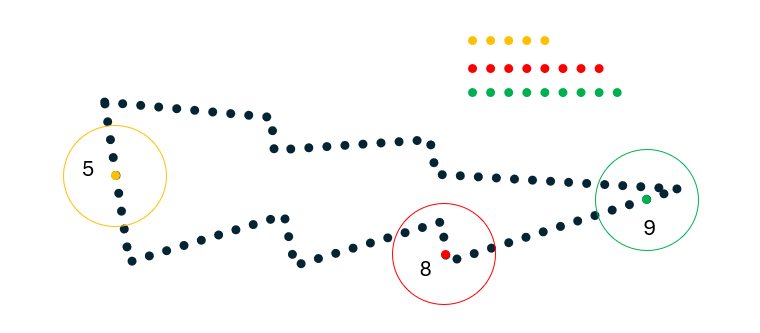
\includegraphics[width=0.5\textwidth]{figures/Points_inside.png}
    \caption{Variation in area density for different geometries on a figure of equal edge density}\label{fig:area_and_circumference}
\end{figure}

The same principle extends to 3D point clouds. Since the points represent the surface, quality should be assessed based on surface density—defined as the number of points per unit surface area. As with area density in 2D, local volume density in 3D offers a simpler, though less accurate, estimate of point cloud quality than true surface density. By placing a Euclidean ball at a point, as illustrated in Figure~\ref{fig:volume_and_surface}, volume density is computed by counting the number of points within the radius. The surface density is yet again closely related, as the number of points inside the radius is the product of surface density and suface area within the radius.

\begin{figure}[H]
    \centering
    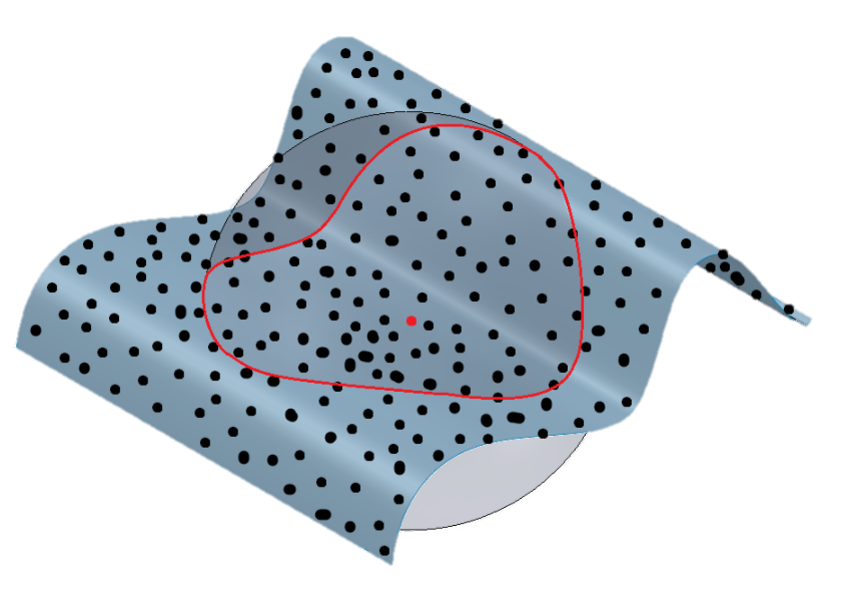
\includegraphics[width=0.5\textwidth]{figures/Surface_volume_density.png}
    \caption{Points inside euclidean ball shows relationsship between volume density and surface density}\label{fig:volume_and_surface}
\end{figure}

Estimating surface area in 3D is considerably more computationally expensive than computing edge length in 2D, and becomes impractical for large-scale point clouds. As in 2D, different surface geometries, such as corners, curves, and flat regions—introduce varying geometry biases. We argue that surface density can be learned by a neural network using local volume density in combination with features that capture the geometry bias.